%----------------------------------------------------------------------------
\chapter{The used cyberphysical system}
%----------------------------------------------------------------------------
\section{Usage of the designed software}

The designed monitoring software is made to be part of the system created for the Future Internet Research, Services and Technology project started by ETIK organization. The system is a prototype of a sensor network where the output of sensors can be used to create so called virtual sensors and store the data in a central data store. The system can reason using the ontology built on the sensors. A detailed introduction can be found in this chapter.

\section{Goal of the project}

The project's goal is to show a prototype of a cyberphisical system. It should contain sample sensors, a central database and also a planner, which plans the deployment of the designed new processes or virtual sensors. The system should prove using small example use cases that such a system is feasible to build. The prototype should not need to scale for large amount of sensors.

\section{System architecture}

The system was designed in the following way: 
There are computing or sensing resources called nodes which can provide computational capacity for the new application or sensor output using its sensors. The measurements are sent to the central SOS server and the available free resource information to the RDF store.
The SOS server stores the measurements and provide the data to the other nodes. There is a translation module, which can create the RDF representation of the sensor database for the ontology. 
The RDF store contains the overall architecture of the deployed applications and resource nodes. It also stores the load of each node. 
There is a sensor browser module which users can use to search in the ontology. It is connected to a measurement browser which will display the observations of the selected sensors. 
Users can deploy new application through the planner system. A package shall be uploaded and the planner should automatically deploy it to the chosen node. 
The status of the system can be seen on the implemented monitoring system.

\begin{figure}[h]
	\centering
	%custom
	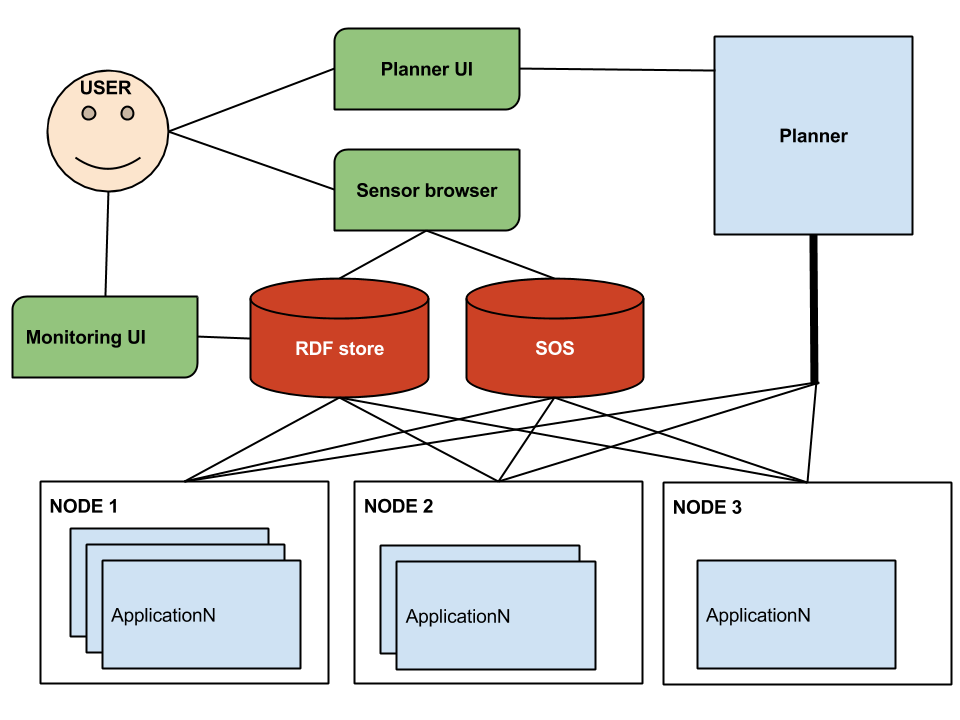
\includegraphics[width=0.6\textwidth]{figures/sysarch.png}
	\caption{System overview\label{fig:sysover}}
\end{figure}

\section{Sensors and resources}
The system is using different devices with different capabilities. There are simple microcontrollers and high performance mobile phones integrated in the system. 

The most simple solution is the Arduino Uno board with ethernet controller. The card has an AVR based microcontroller working inside. It is good for simple measurement. 

The next in computational power is the Beagle Board. 